\chapter{Magnetik}

\section{Das Erdmagnetfeld}
\subsection{Aufbau}

Das Erdmagnetfeld lässt sich in drei Bereiche unterteilen. 


\begin{figure}[H]
	\centering
	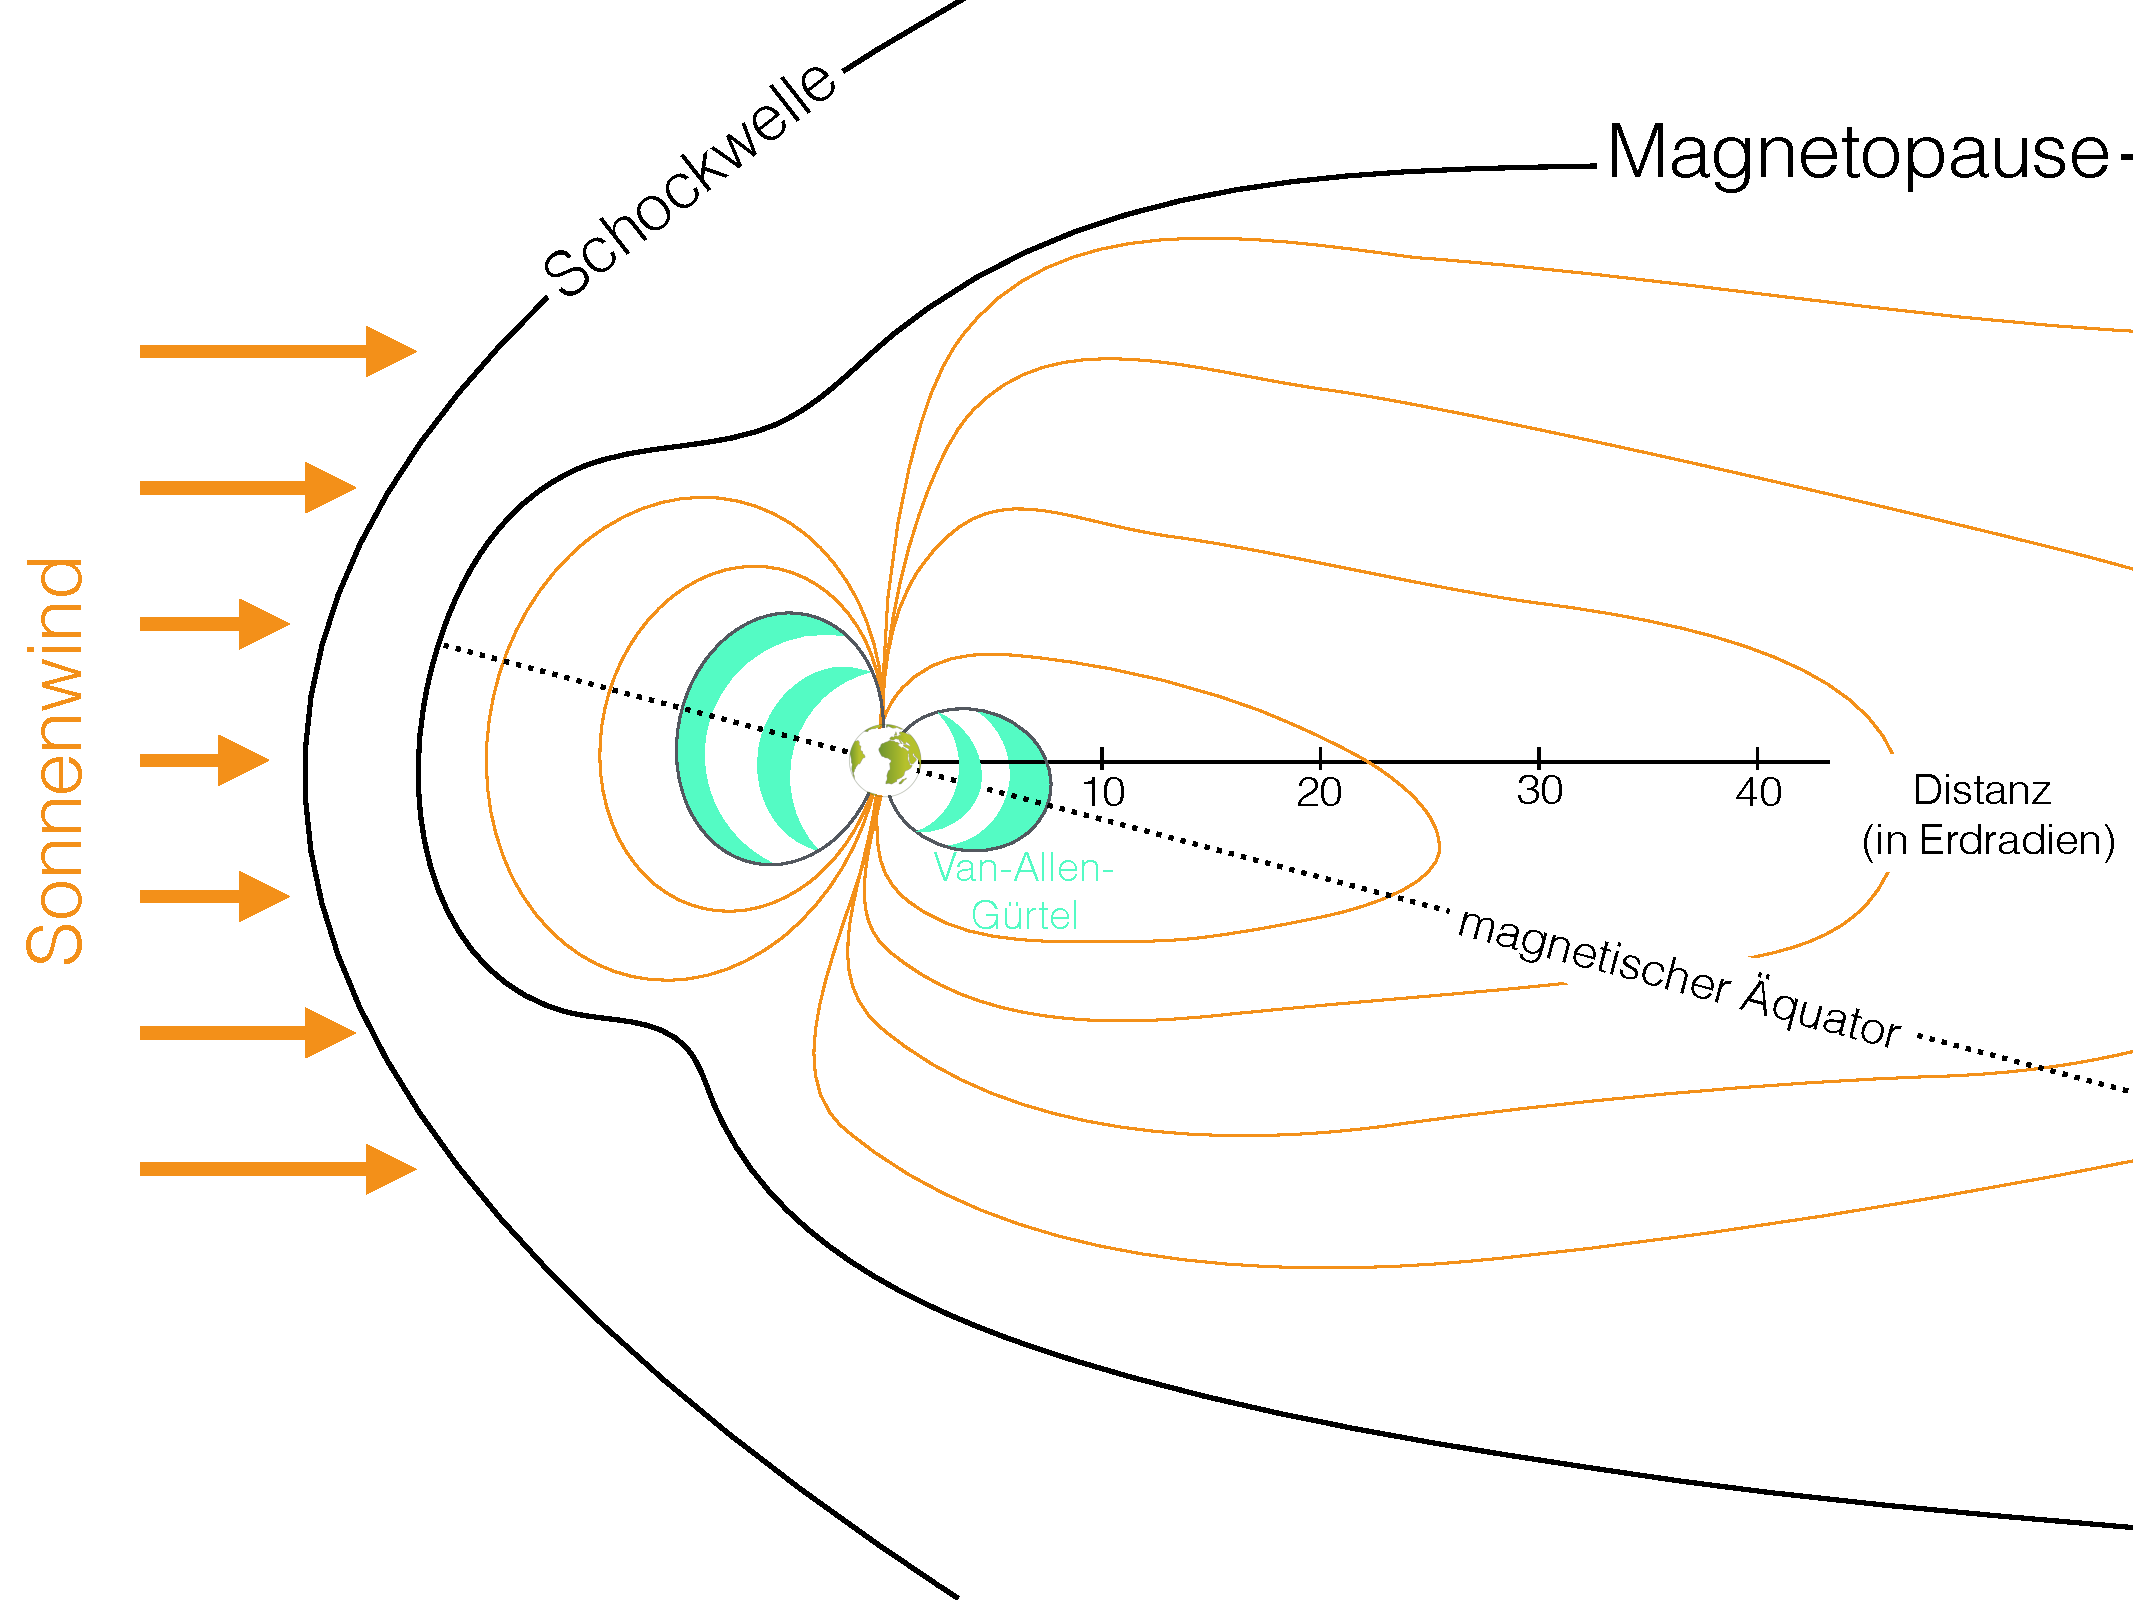
\includegraphics[width = \textwidth]{MagnetikBilder/Erdmagnetfeld}
\end{figure}

\subsubsection{Das Außenfeld: Magnetosphäre}
Auf diese äußere magnetische Hülle treffen elektrisch geladene Teilchen des Sonnenwindes mit einer relativen Geschwindigkeit von 400\,m/s. Durch diese hohe Geschwindigkeit bildet sich eine Schock-Welle, die \textbf{Magnetopause}, auf der sonnennahen Erdseite.
Die auftreffenden Teilchen des Sonnenwindes verursachen Magnetfelder. Das Erdmagnetfeld wird aufgrund der Sonnenwinde auf der Tagseite verstärkt und auf der Nachtseite abgeschwächt.

Die Feldlinien der Magnetosphäre bilden eine tränenartige Form, die sich bis zu 50\,000\,km (etwa 8 Erdradien) erstreckt.

\subsubsection{Van-Allen-Gürtel: 2000 -- 20\,000 km}
Die Ionen des Sonnenwindes und der Ionosphäre werden im Magnetfeld gefangen. Entlang magnetischer Linien wandern diese schraubenartig von Pol zu Pol. Dabei bilden sich Gürtel mit intensiver Strahlung, der Van-Allen-Gürtel.\begin{itemize}
	\item innerer Gürtel: 2000 -- 5000 km Höhe
	\item äußerer Gürtel: 13\,000 -- 20\,000 km Höhe
\end{itemize} 
Die magnetischen Effekte auf der Erdoberfläche sind aufgrund der großen Entfernung jedoch gering. Sichtbar werden die Gürtel aber dennoch, wenn es zu einer Überladung der Gürtel kommt. Dann streifen die Partikel die obere Atmosphäre und regen diese zu Floureszenz an, was dann als Polarlichter sichtbar wird.

\begin{figure}[H]
	\centering
	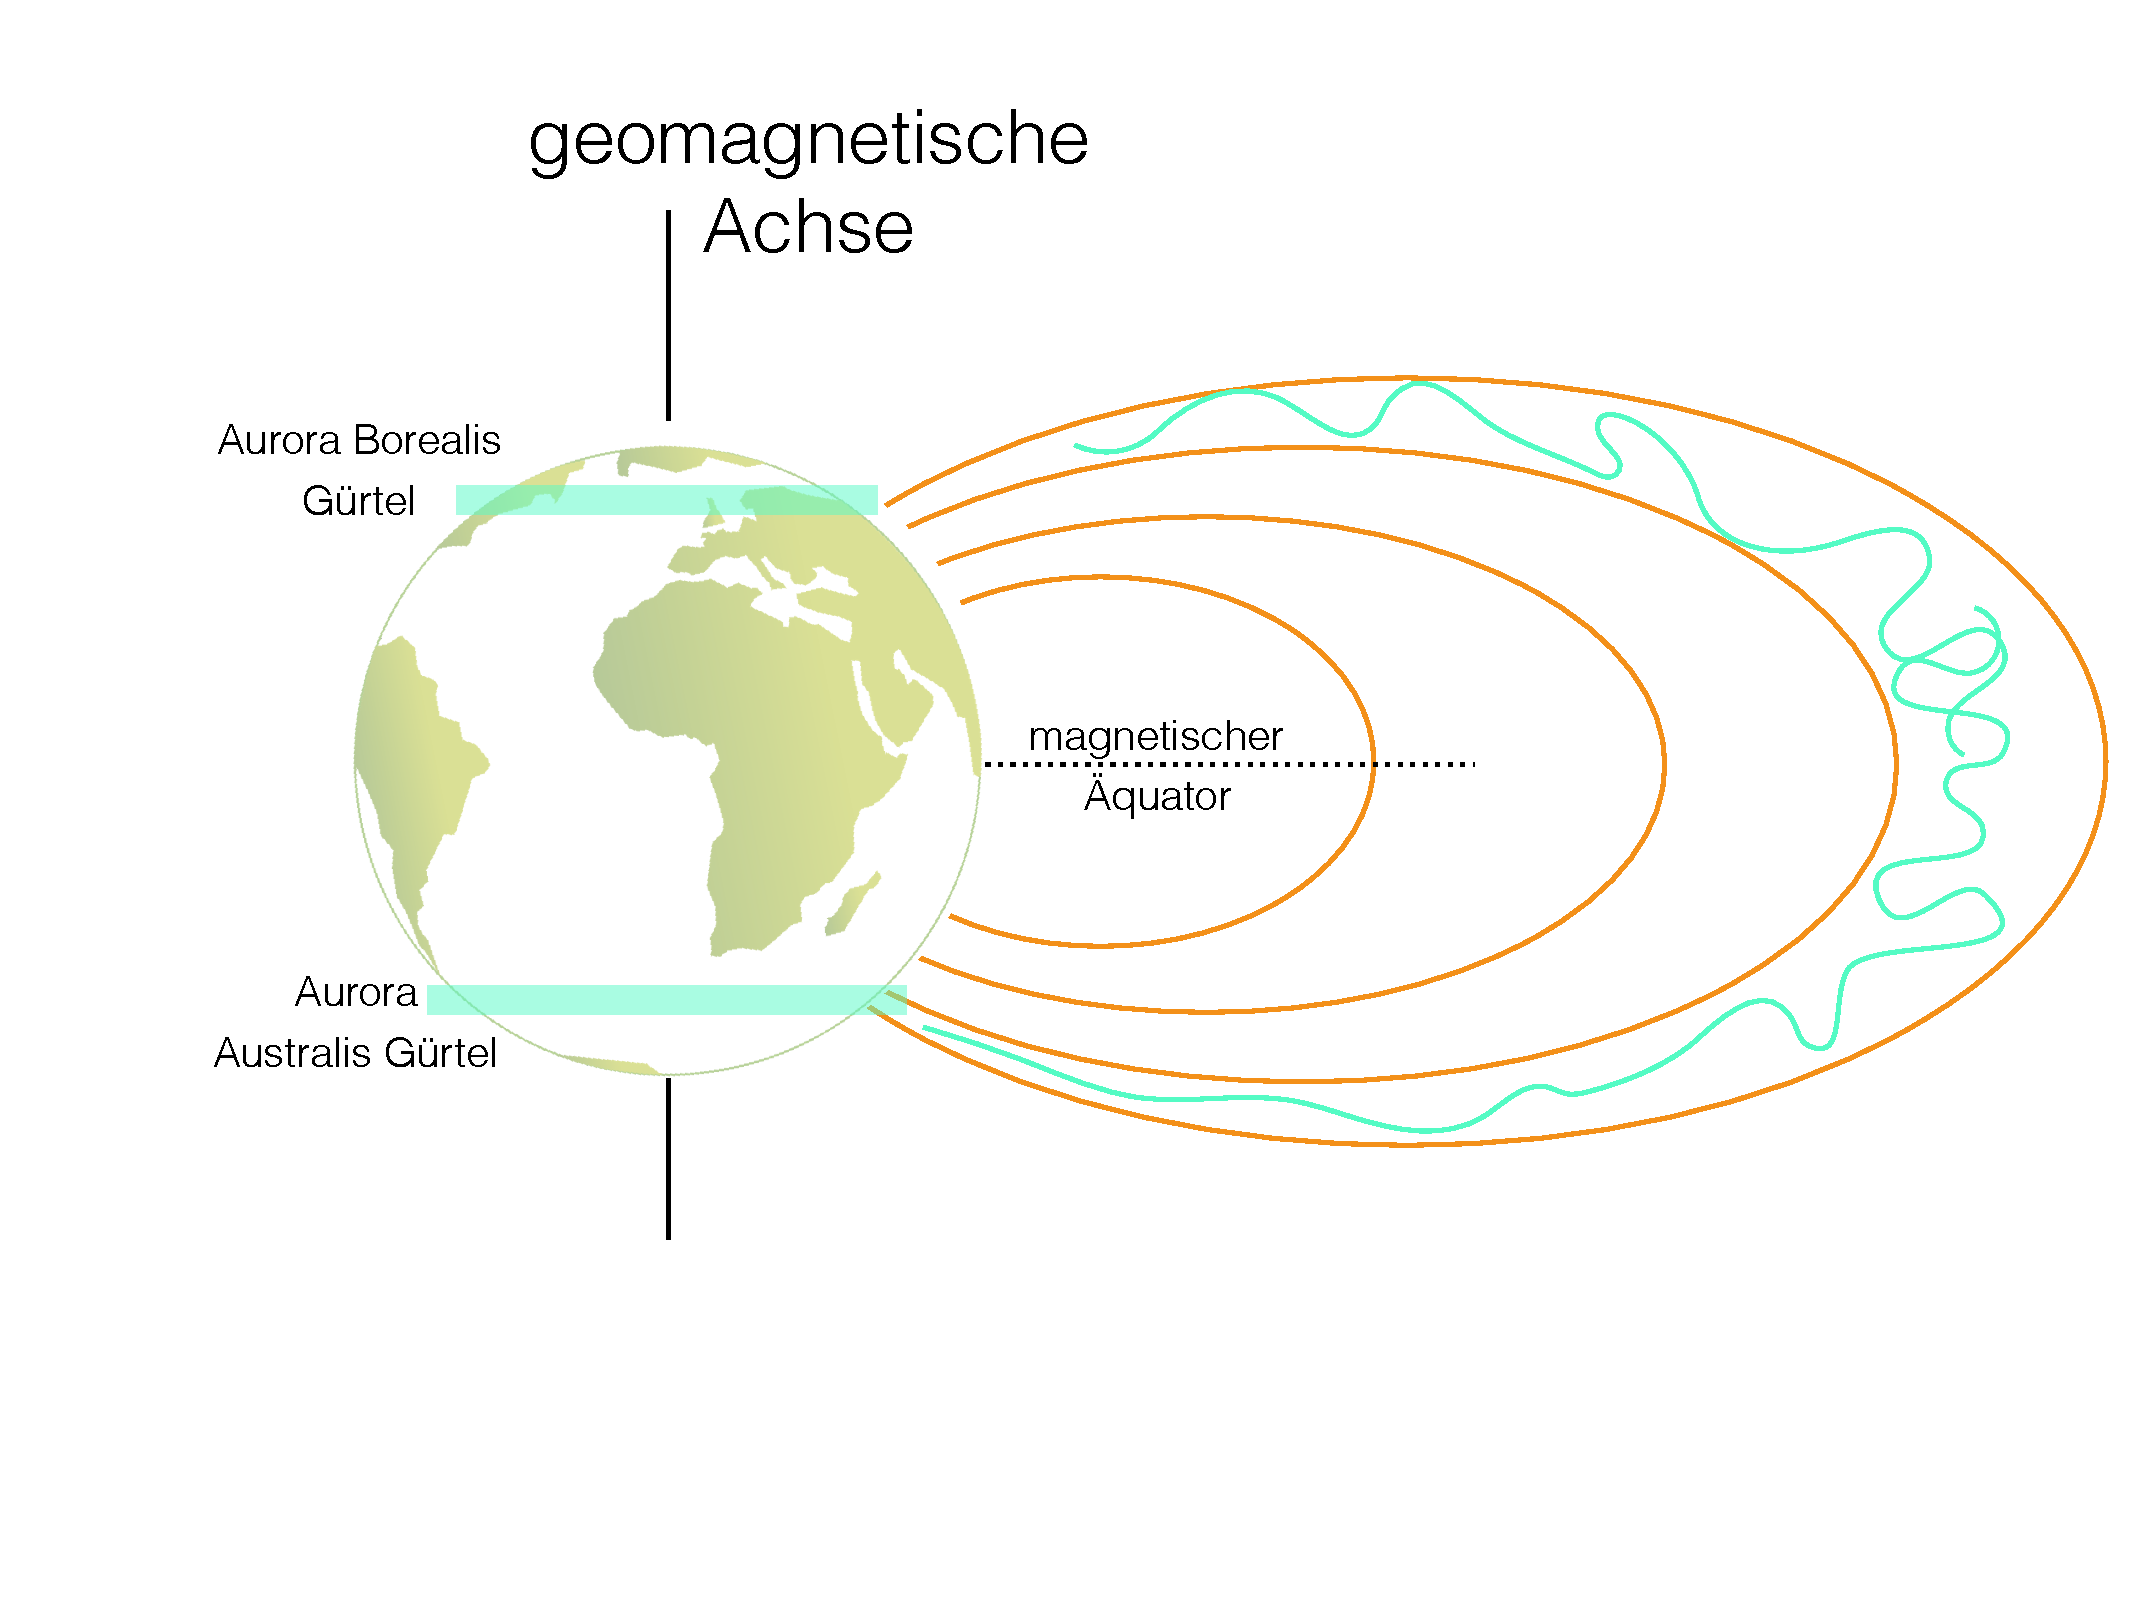
\includegraphics[width = \textwidth]{MagnetikBilder/VanAllenGuertel}
\end{figure}


\subsubsection{Ionosphäre: 80 -- 500 km}
Die UV-Strahlung der Sonne ionisiert Moleküle der oberen Atmosphäre. Diese setzten Elektronen frei, welche sich der Feldlinien entlang bewegen. Durch diese Bewegung bilden sich Stromkreise, die wiederum Magnetfelder erzeugen.
Dieses Feld ist schließlich das "`spürbare Außenfeld"' an der Erdoberfläche.

\subsection{Variationen des Erdmagnetfeldes}
Das Erdmagnetfeld untersteht einem ständigen, zeitlich abhängigen Wandel durch Umwelteinflüsse.

\subsubsection{Tägliche Variationen}
Die Magnetfelder der Ionosphäre schwanken aufgrund der Erddrehung im Laufe eines Tages.
Sonnenflecken und Sonnenwinde (magnetische Stürme) lösen eine starke Strahlung aus, welche das Erdmagnetfeld verstärken. Diese haben Intensitäten bis zu 1000 nT. Diese tägliche Variation des Erdmagnetfeldes ist breitenabhängig, wobei sie an den Polen stärker ist.

\subsubsection{Längerfristige Variationen}
Das Erdmagnetfeld variiert nicht nur im Laufe eines Tages, sondern hat auch deutlich langwierigere Veränderungen. Zum Beispiel kehrt sich das Magnetfeld mit Perioden von $10^{12}$ Sekunden (knapp 2 Milliarden Jahre) um. Auch die \textbf{Säkularvariationen} (Variationen der Polstärken) haben eine sehr lange Periode von $10^9$ -- $10^{10}$ Sekunden.

\subsection{Beschreibung des Magnetfeldes}
\subsubsection{Näherung: Dipolfeld}
In erster Näherung entspricht das Erdmagnetfeld einem Dipolfeld. Die Achse des Feldes ist gegenüber der Rotationsachse der Erde um 11,4 -- 11,5$^{\circ}$ geneigt. 
Die Dipolintenistät ist allerdings nicht konstant, sie ist an den Polen stärker: \begin{description}
	\item Äquator: $\approx$ 30 000 nT
	\item Nordpol: $\approx$ 60 000 nT
	\item Karlsruhe: $\approx$ 47 000 nT
\end{description}

\begin{figure}[H]
	\centering
	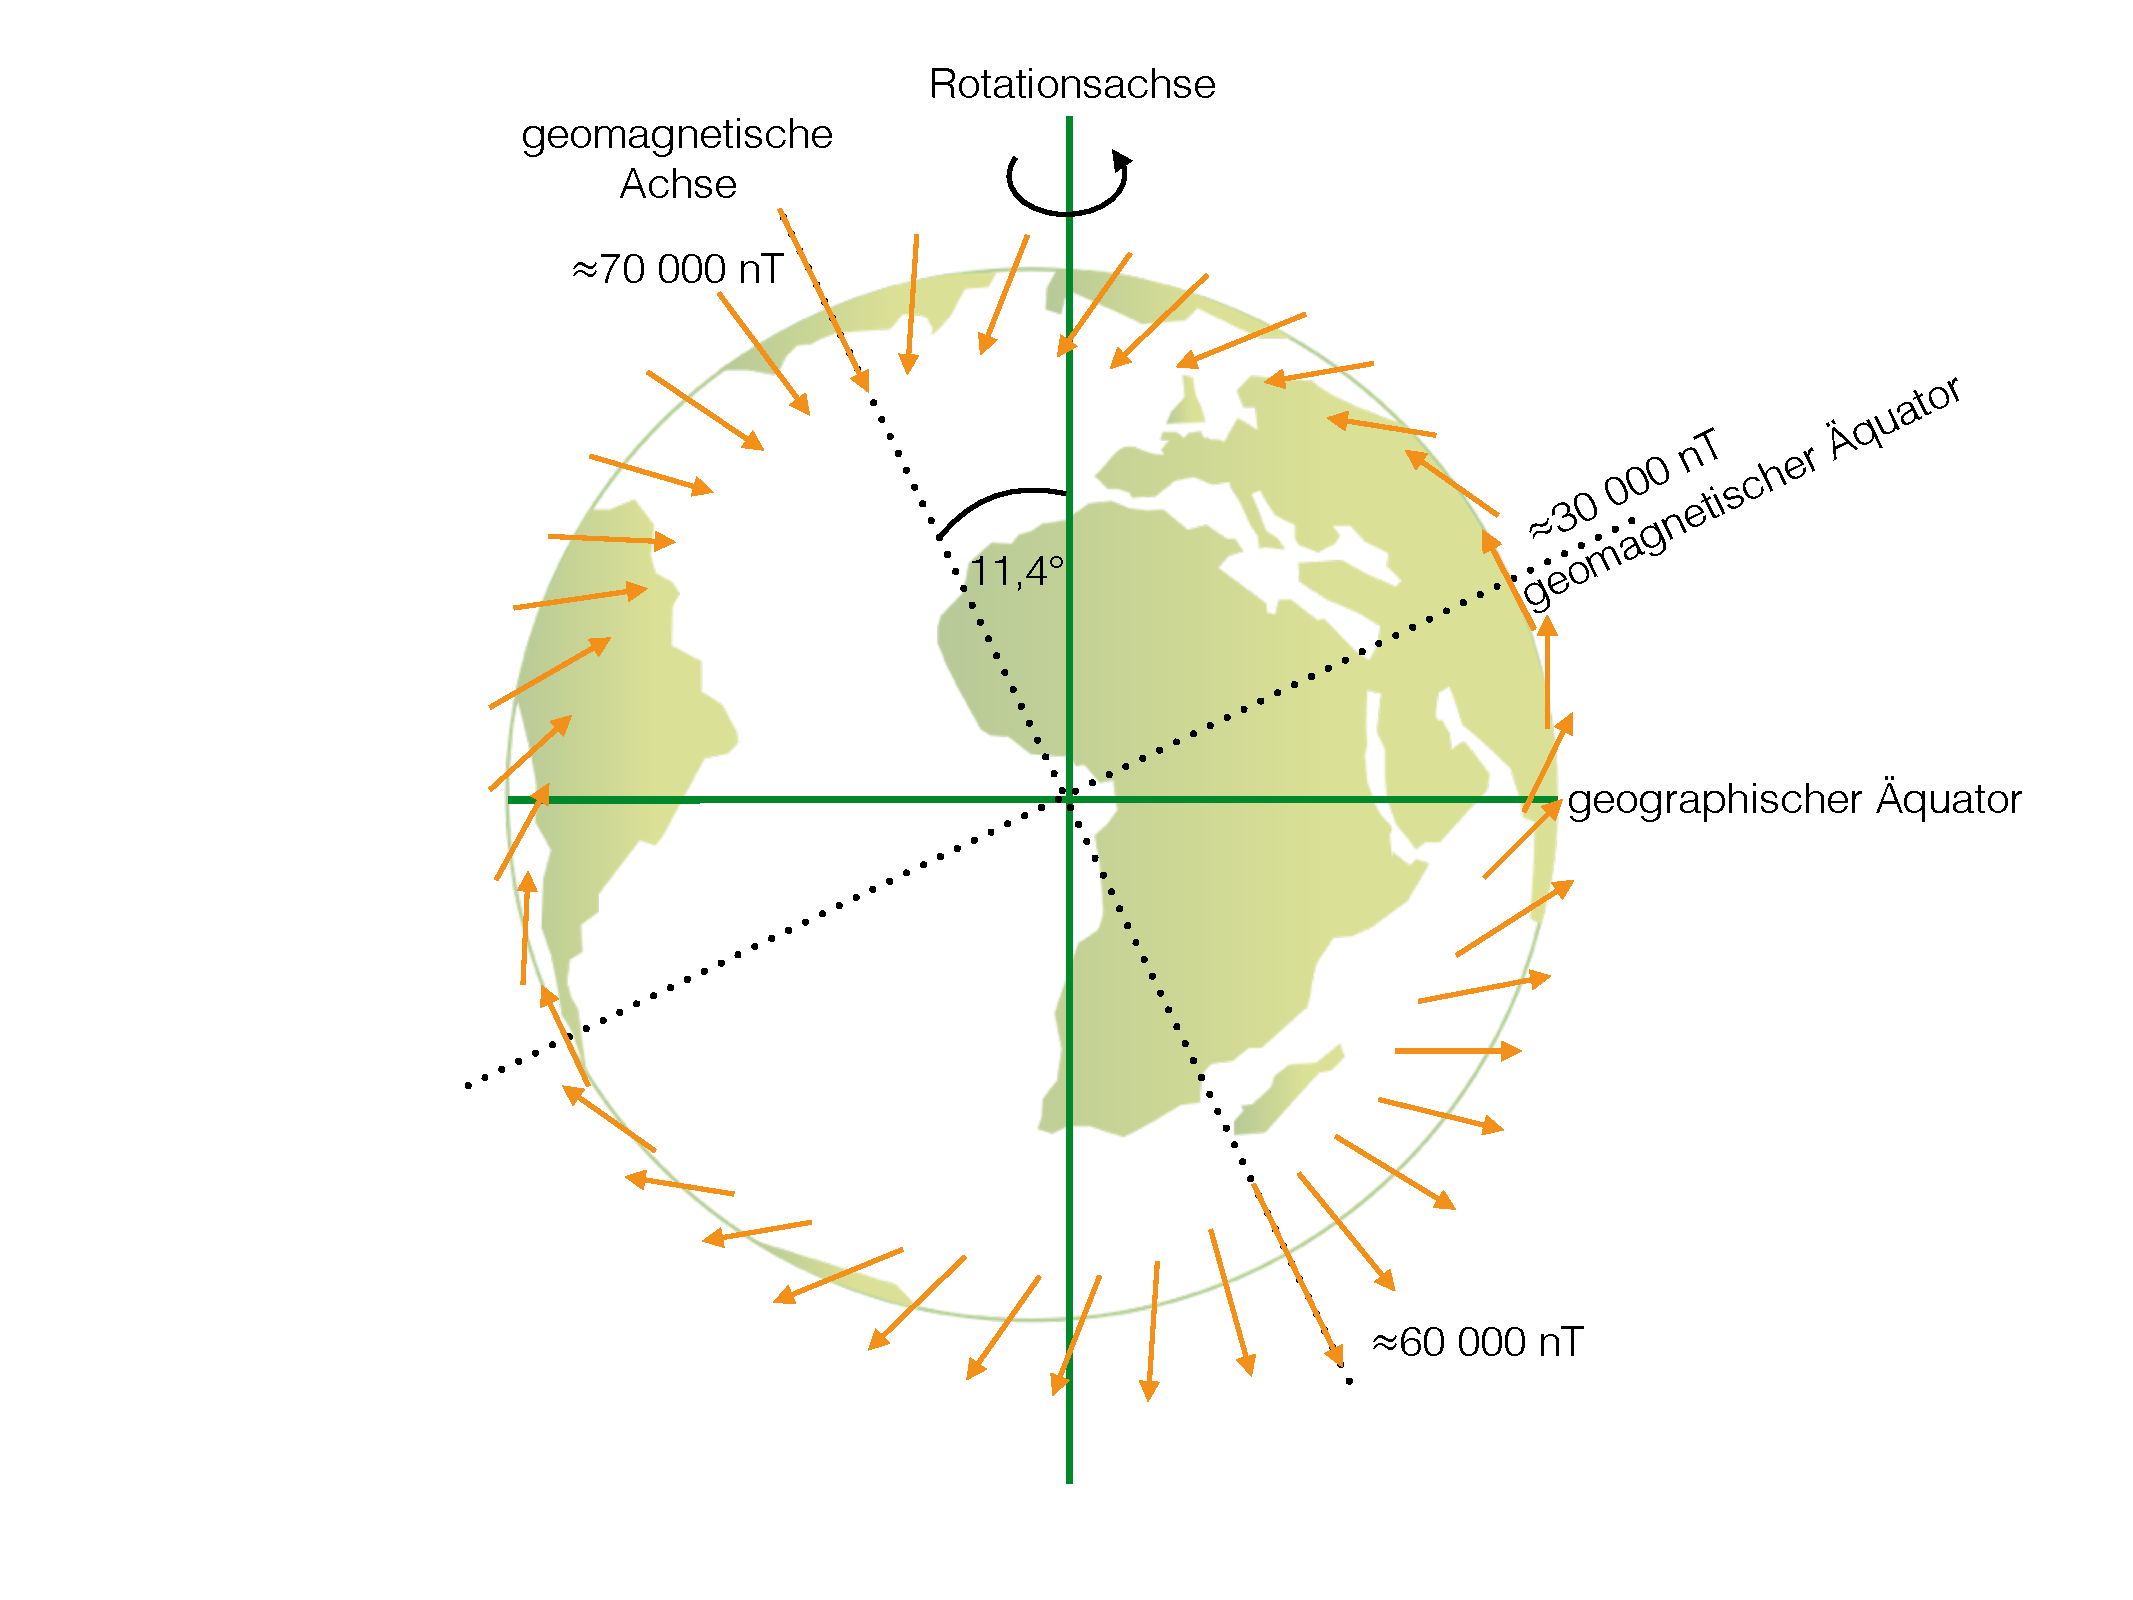
\includegraphics[width = \textwidth]{MagnetikBilder/Dipolfeld}
\end{figure}


\subsubsection{Nichtdipolfeld}
Zwar lässt sich das Erdmagnetfeld als Dipolfeld nähern, aber es gibt dennoch starke Abweichungen davon. Das Nichtdipolfeld ist ein System aus wirbelförmigen Anomalien. Um jeden Breitenkreis treten etwa 1 -- 2 positive und 1 -- 2 negative solcher Anomalien auf. Der Grund warum wir auf diese Anomalien überhaupt eingehen, ist ihre Stärke. Solche Anomalien können bis zu 20 000 nT betragen. Das Nichtdipolfeld ändert sich zum Teil mit der Zeit, allerdings gibt es auch einen stationären Anteil. Diese Änderungen sind die Säkularvariationen.



\subsection{Mathematische Beschreibung}
Wir wollen uns in diesem Abschnitt das Erdmagnetfeld auf etwas mathematischere oder physikalischere Weise anschauen.

Dazu betrachten wir zunächst einige physikalischen Grundlagen zum Thema Magnetfeld. 

Wir beginnen mit der Berechnung des Feldes eines Dipols, mit Hilfe folgender Grafik:


\begin{figure}[H]
	\centering
	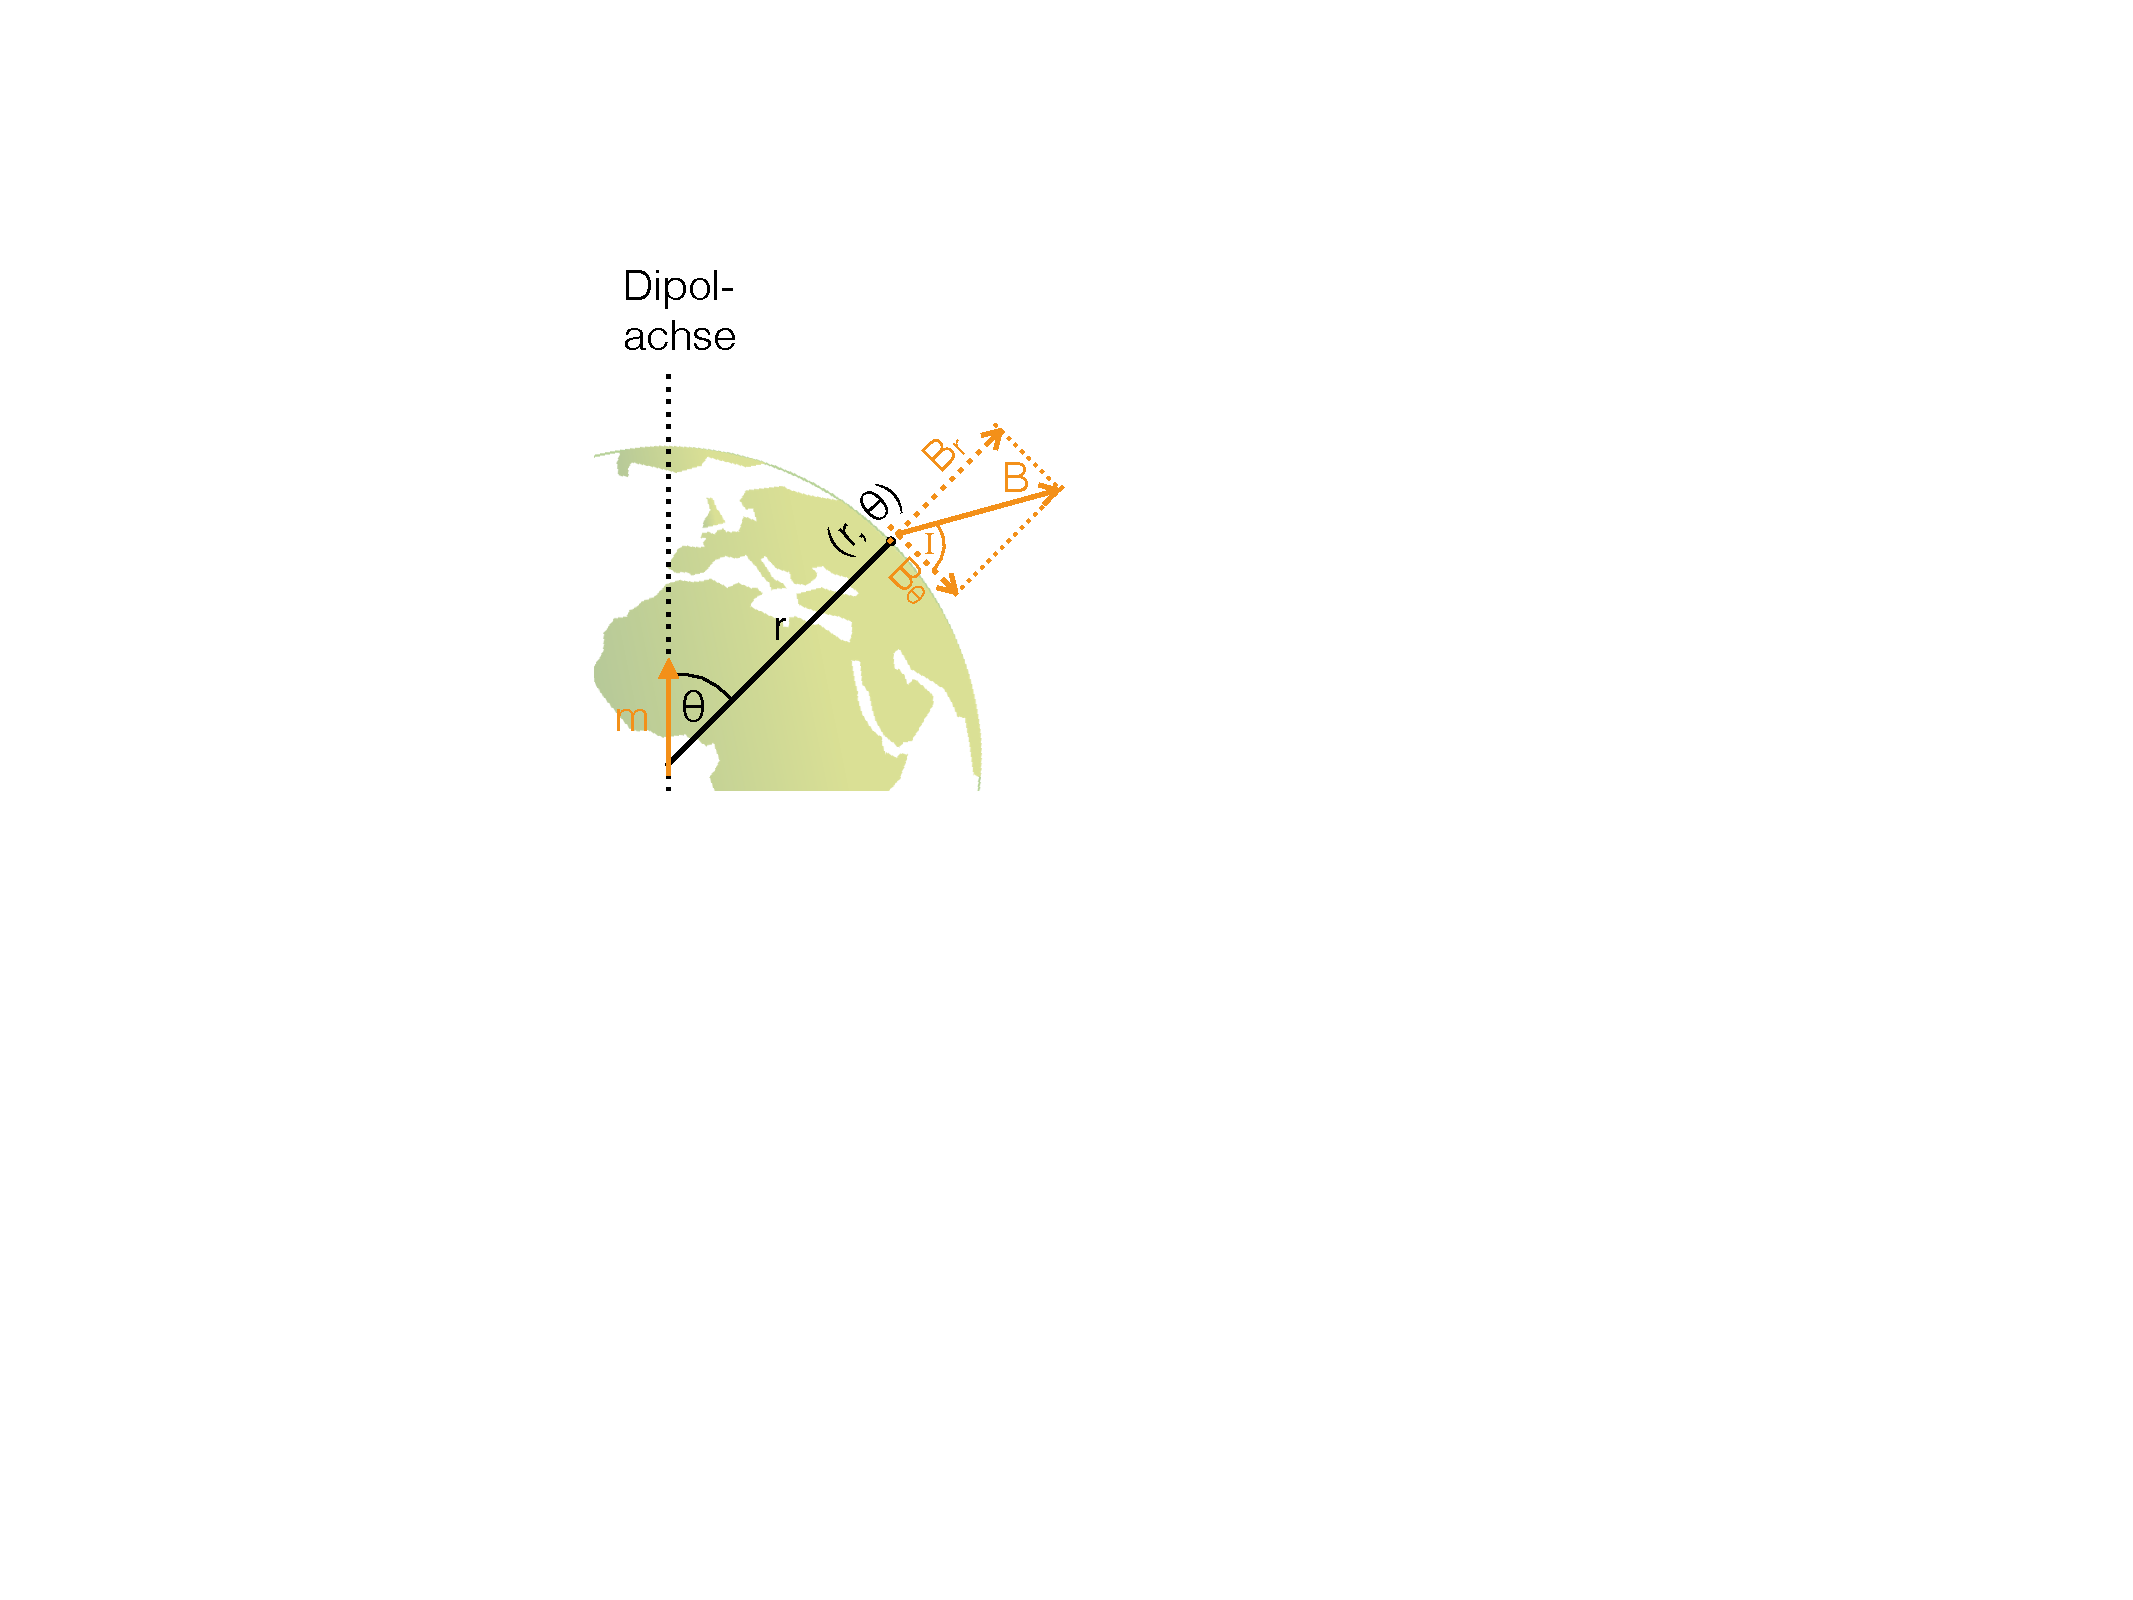
\includegraphics[scale = 0.6]{MagnetikBilder/PotentialDipol}
\end{figure}


 
Weiterhin werden wir ohne Herleitung die Formel zur Berechnung des Dipolpotentials verwenden: \begin{equation*}
	W = \frac{\mu_0}{4 \cdot \pi} \cdot \frac{m \cdot cos(\theta)}{r^2} \quad \text{mit } \mu_0 = 4 \cdot \pi \cdot 10^{-7}\,\si{\frac{N}{A^2}}
\end{equation*}
$\mu_0$ heißt magnetische Feldkonstante und $m$ ist das magnetische Moment. Letzteres gibt die Stärke des Dipolfeldes an.

Das Dipolfeld lässt sich nun in eine radiale Komponente $B_r$ und eine transversale Komponente $B_{\theta}$. Diese berechnen sich folgendermaßen: \begin{align*}
	B = (B_r, B_{\theta}) = \begin{cases}
		B_r = - \dfrac{dW}{dr} = \dfrac{\mu_0}{4 \cdot \pi} \cdot \dfrac{2 \cdot m \cdot cos(\theta)}{r^3} \\
		B_{\theta} = - \dfrac{1}{r} \dfrac{dW}{d \theta} = \dfrac{\mu_0}{4 \cdot \pi} \cdot \dfrac{m \cdot sin(\theta)}{r^3}
	\end{cases}
\end{align*}


Mit der Information zur Berechnung der Feldkomponenten lassen sich nun zwei Feldelemente beschreiben, welche die Richtung des magnetischen Feldes bezüglich des lokalen Koordinatensystems angeben.

\subsubsection{Inklination}
Die Inklination gibt an, in welchem Winkel die magnetischen Feldlinien auf die Erdoberfläche treffen. Der Winkel ist im Bezug zum Horizont. Eine positive Inklination bedeutet, dass die Feldlinien "`nach unten"' geneigt sind. Dies ist (aktuell) in der nördlichen Hemisphäre der Fall. Eine negative Inklination bezeichnet man auch als "`südlich"'. Die Inklination am Äquator ist nahezu 0$^{\circ}$ und in Karlsruhe etwa 63$^{\circ}$.

\begin{figure}[H]
	\centering
	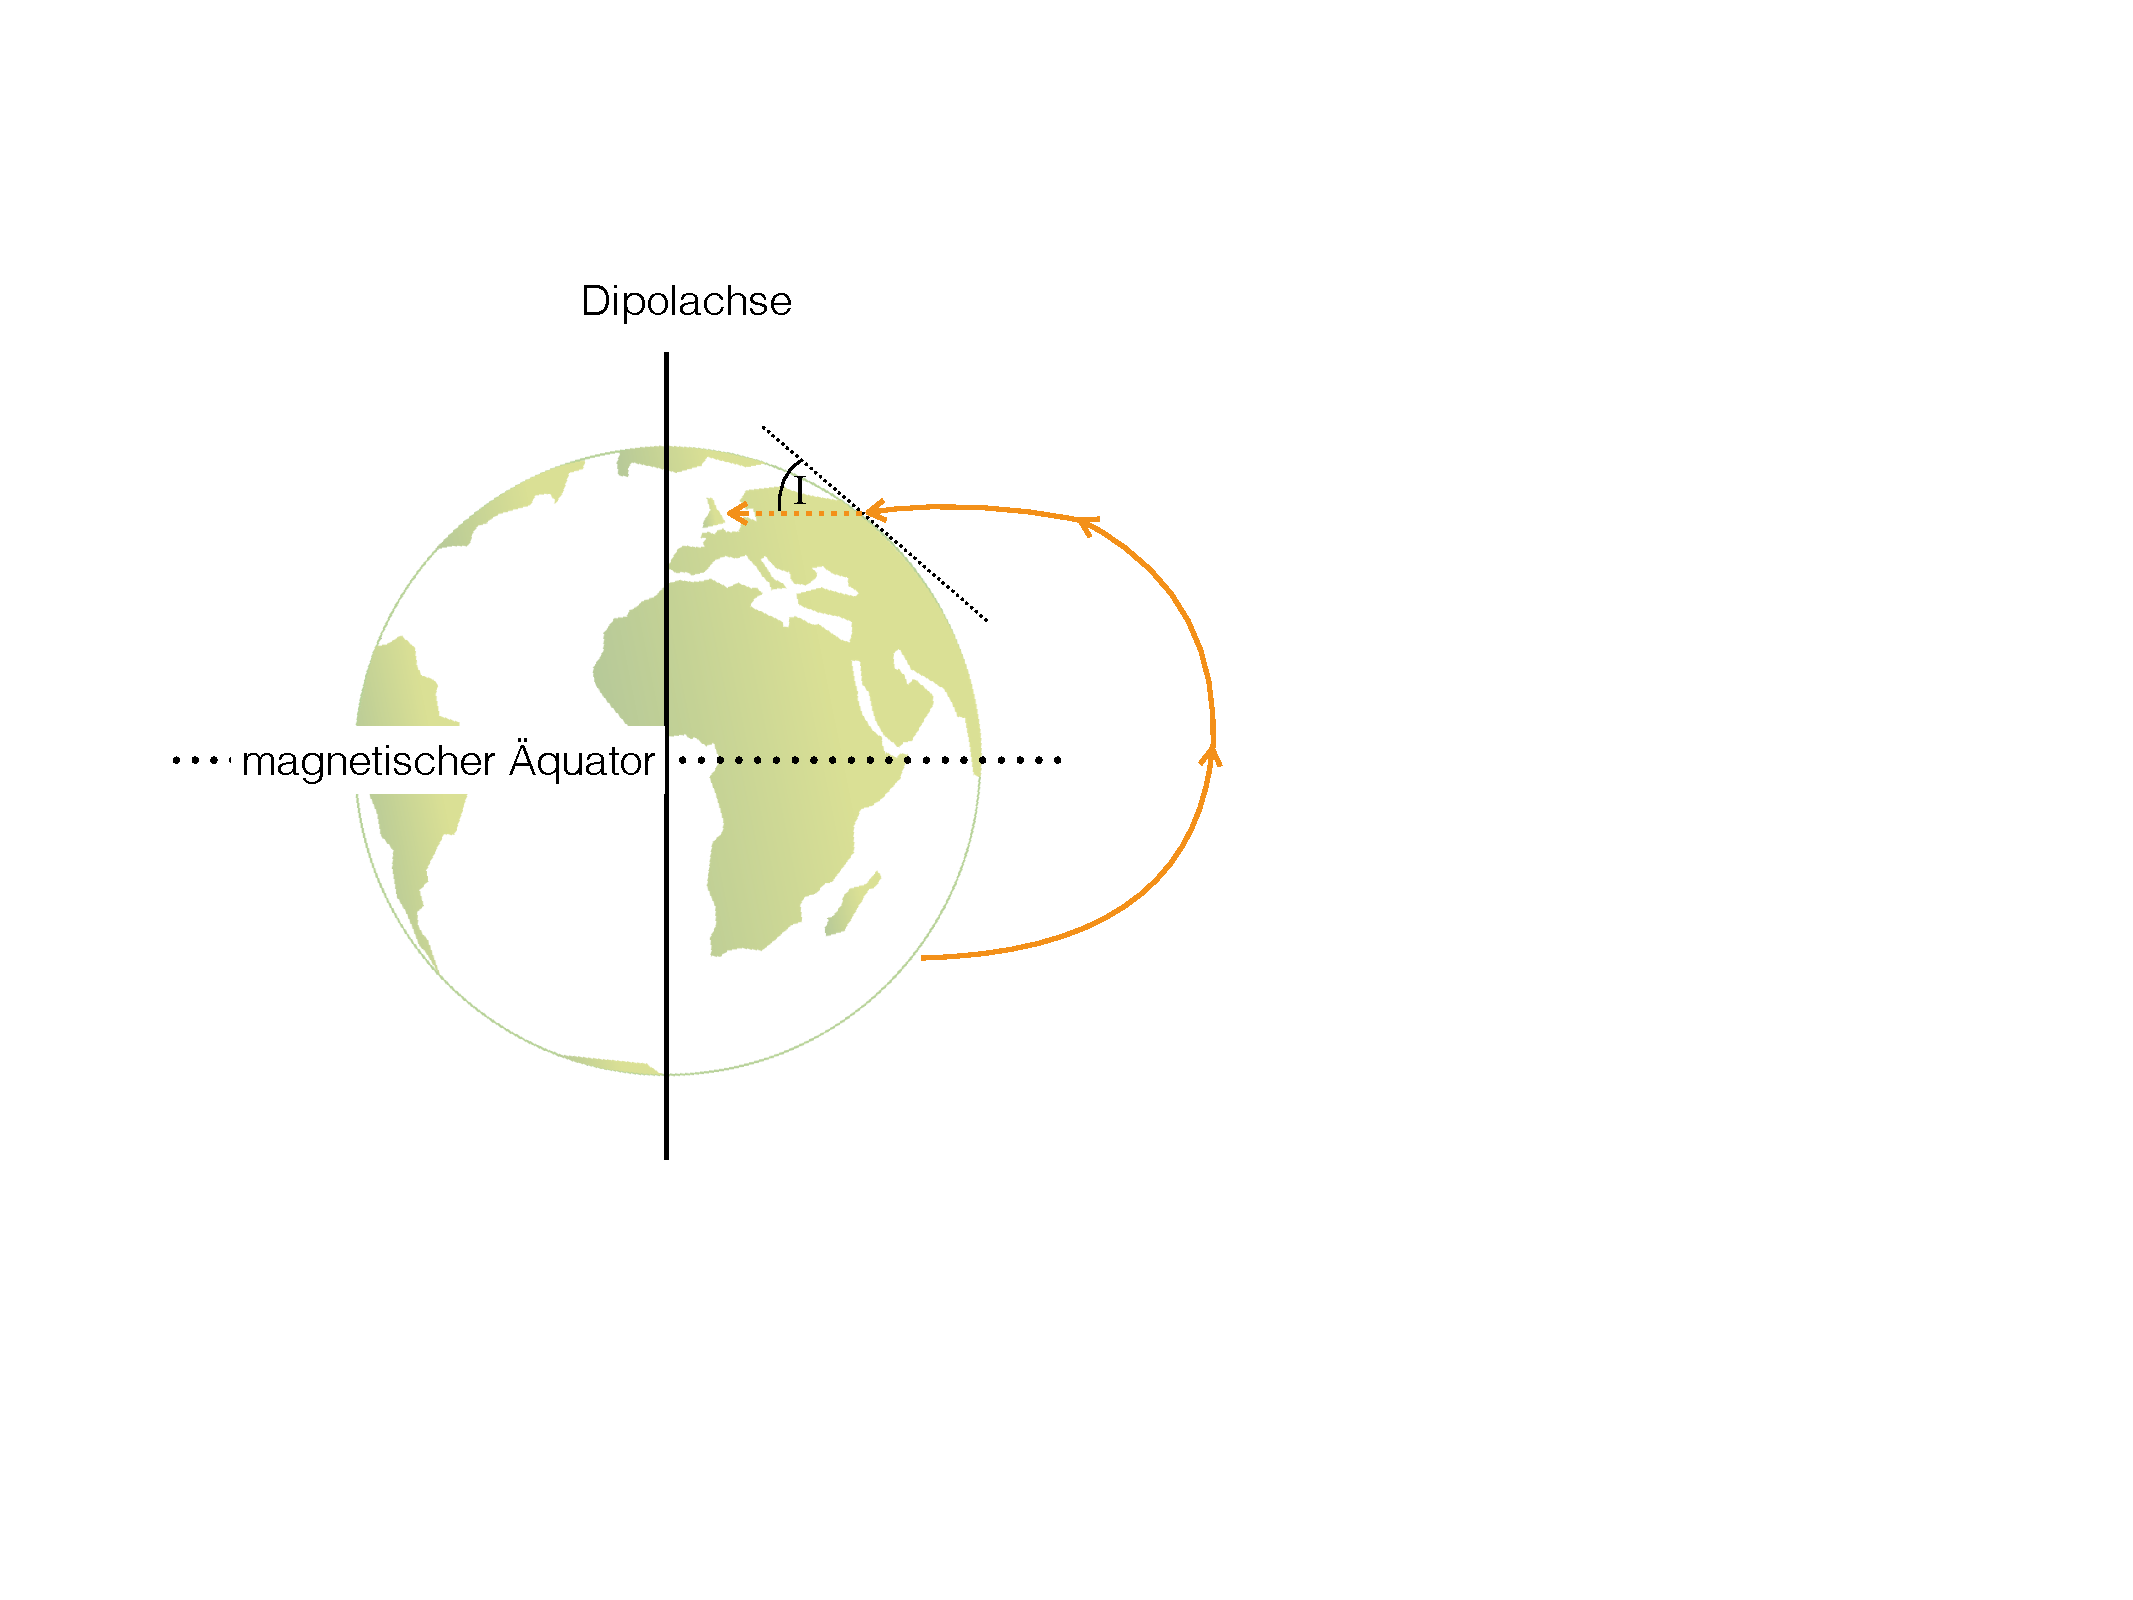
\includegraphics[scale = 0.4]{MagnetikBilder/Inklination}
\end{figure}


\subsubsection{Magnetisch Nord und geomagnetisch Nord}
Obwohl die Begriffe sehr ähnlich sind, unterscheiden sie sich doch deutlich in ihren Bedeutungen. Die magnetischen Pole sind sind die Orte, an denen die Feldlinien senkrecht auf die Erde treffen, die Inklination also 90$^\circ$ beträgt. Die geomagnetischen Pole hingegen geben an, an welcher Stelle die gedachte Dipolachse die Erdoberfläche schneidet. Aufgrund der Säkularvariationen sind beide nicht ortsgebunden, was allgemein unter Polwanderung bekannt ist. Die Konvention ist, den magnetischen Pol der Nordhalbkugel als Nordpol, und den magnetischen Pol der Südhalbkugel als Südpol zu bezeichnen. 


\begin{figure}[H]
	\begin{subfigure}[m]{0.5\textwidth}
	\centering
		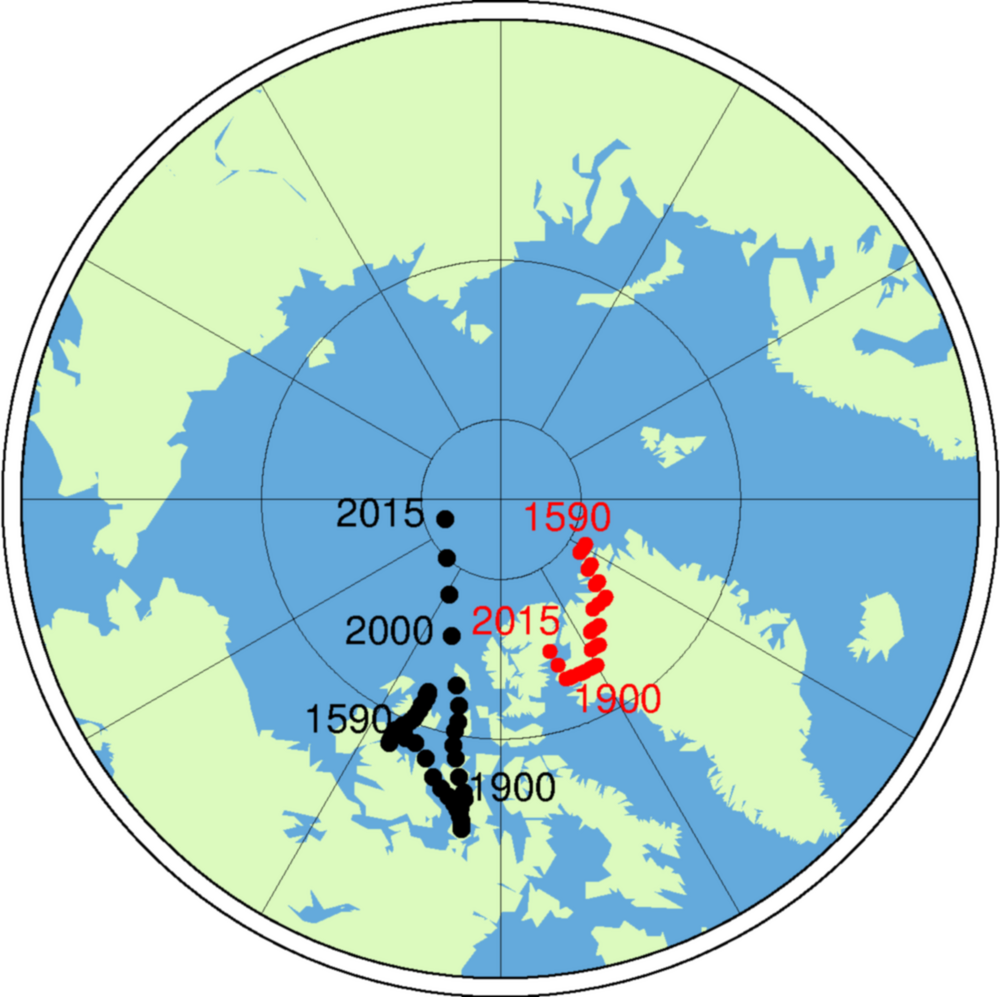
\includegraphics[scale = 0.7]{MagnetikBilder/PowanderungNordpol}	
	\end{subfigure}
	\begin{subfigure}[m]{0.5\textwidth}
	\centering
		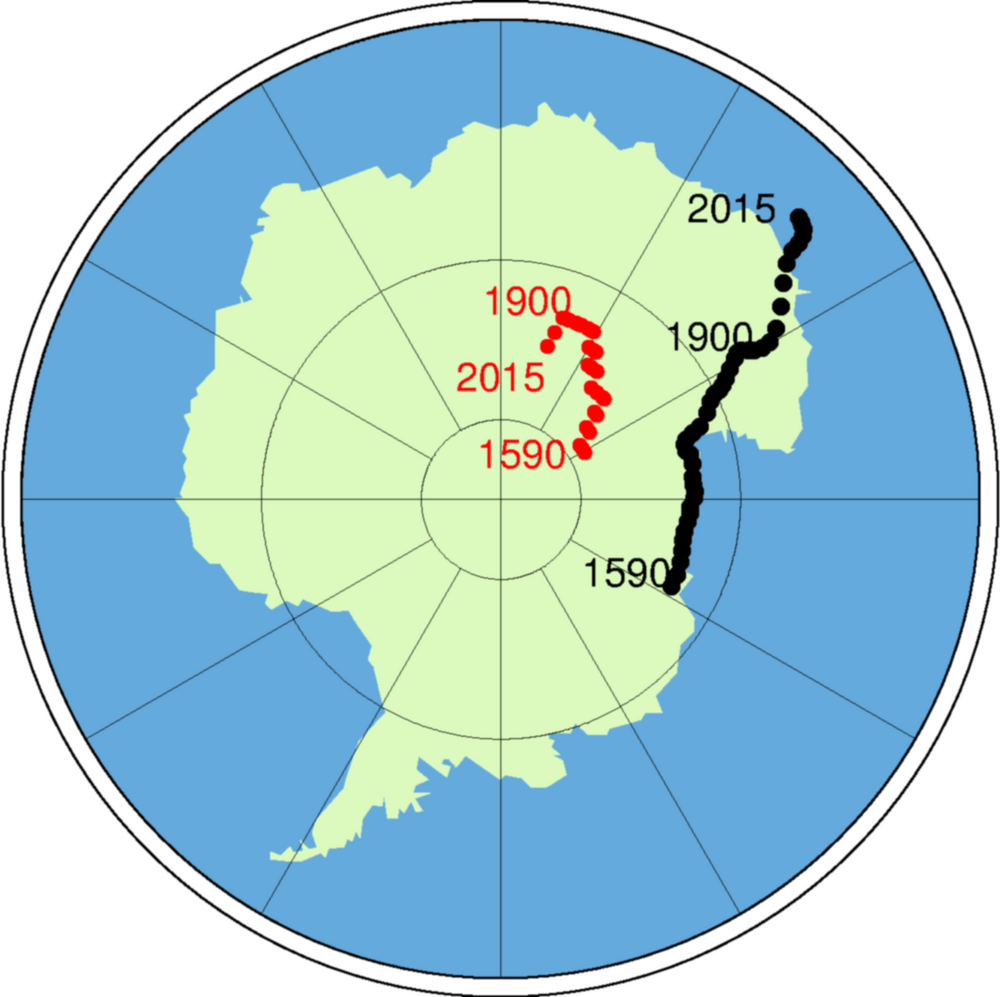
\includegraphics[scale = 0.7]{MagnetikBilder/PolwanderungSuedpol}
	\end{subfigure}
	
	\caption*{Links die Polwanderung auf der Nordalbkugel und rechts auf der Südhalbkugel. Die schwarzen Punkte zeigen die Wanderung des magnetischen Pols an, die roten die Wanderung des geomagnetischen Pols. \textsl{Quelle: Deutsches GeoForschungsZentrum GFZ}}
\end{figure}


\subsubsection{Deklination}
Ein Kompass funktioniert mit Hilfe des Magnetfeldes. Deshalb zeigt auch die Kompassnadel nach dem magnetischen Südpol (aufgrund der Konvention bezeichnen wir diesen Punkt dennoch als "`magnetisch Nord"'). Wo genau dieser Punkt "`magnetisch Nord"' liegt ändert sich mit der Zeit. Wichtig dabei ist, dass sich der geographische Nordpol nicht verändert, da er durch die Rotationsachse der Erde bestimmt ist. Die Deklination ist nun der Winkel zwischen geomagnetisch und geographisch Nord. 
\begin{figure}[H]
	\centering
	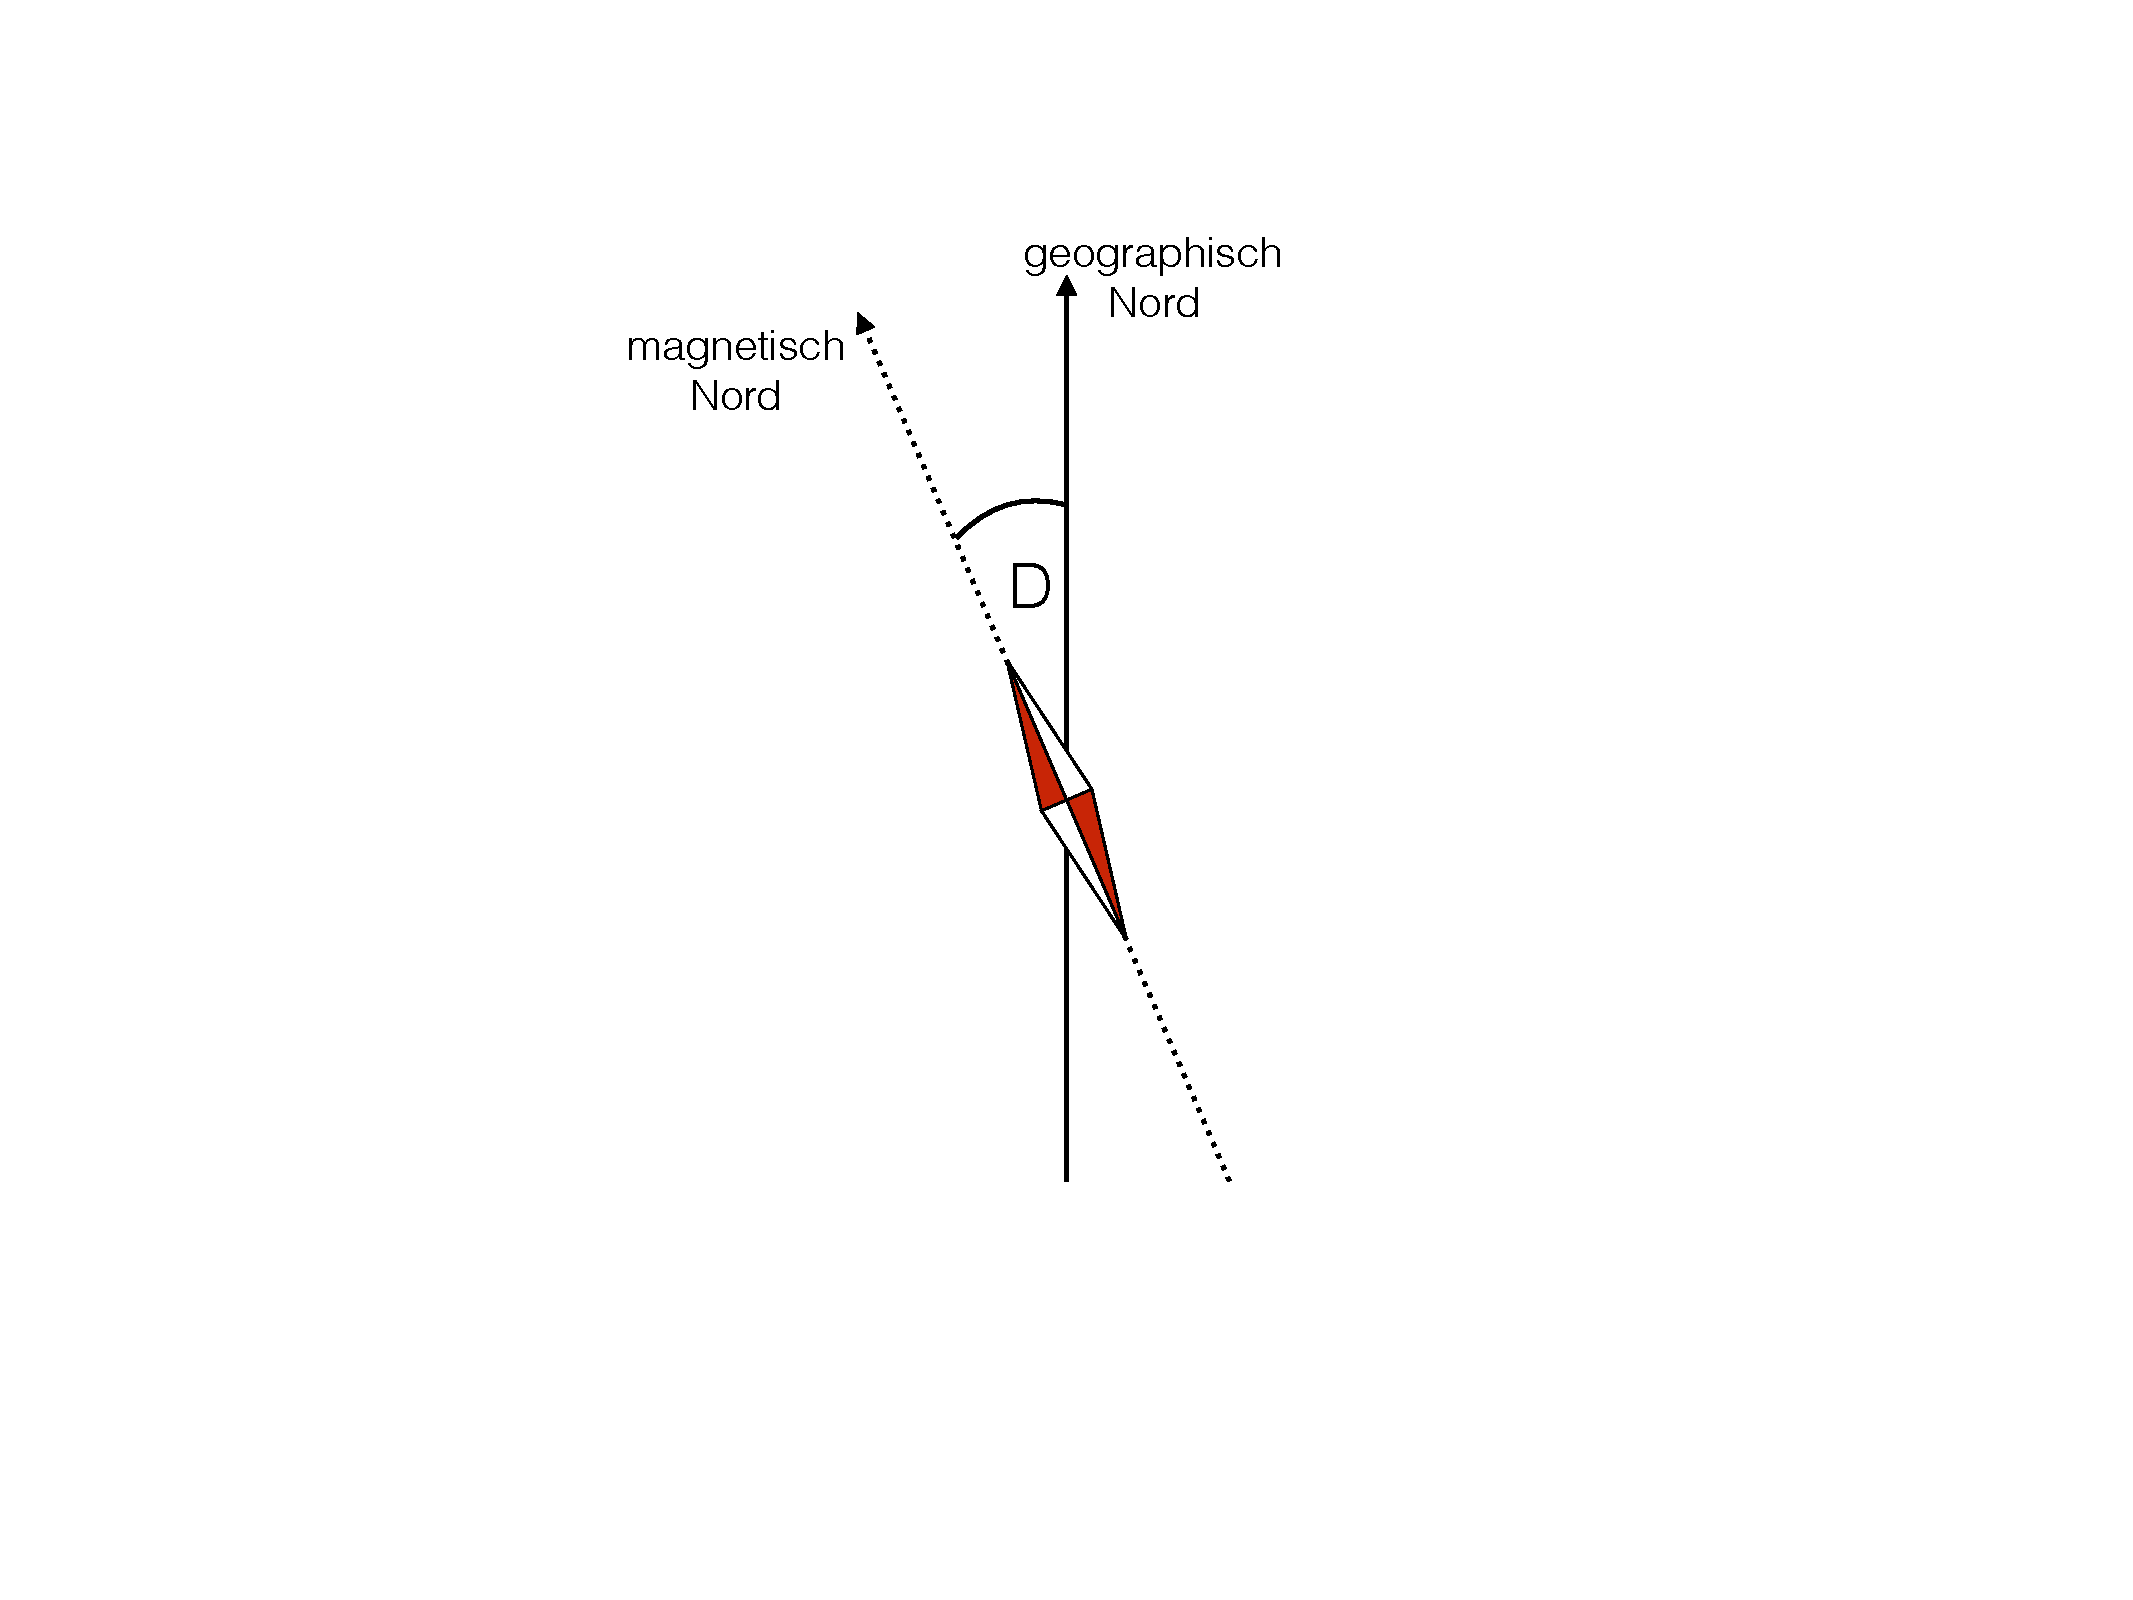
\includegraphics[scale = 0.4]{MagnetikBilder/Deklination}
\end{figure}


\section{Geomagnetische Messungen}
\subsection{Geomagnetische Feldelemente}
Zu Beginn wollen wir uns einmal die Messgrößen einer geomagnetischen Messung anschauen.

\begin{figure}[H]
	\centering
	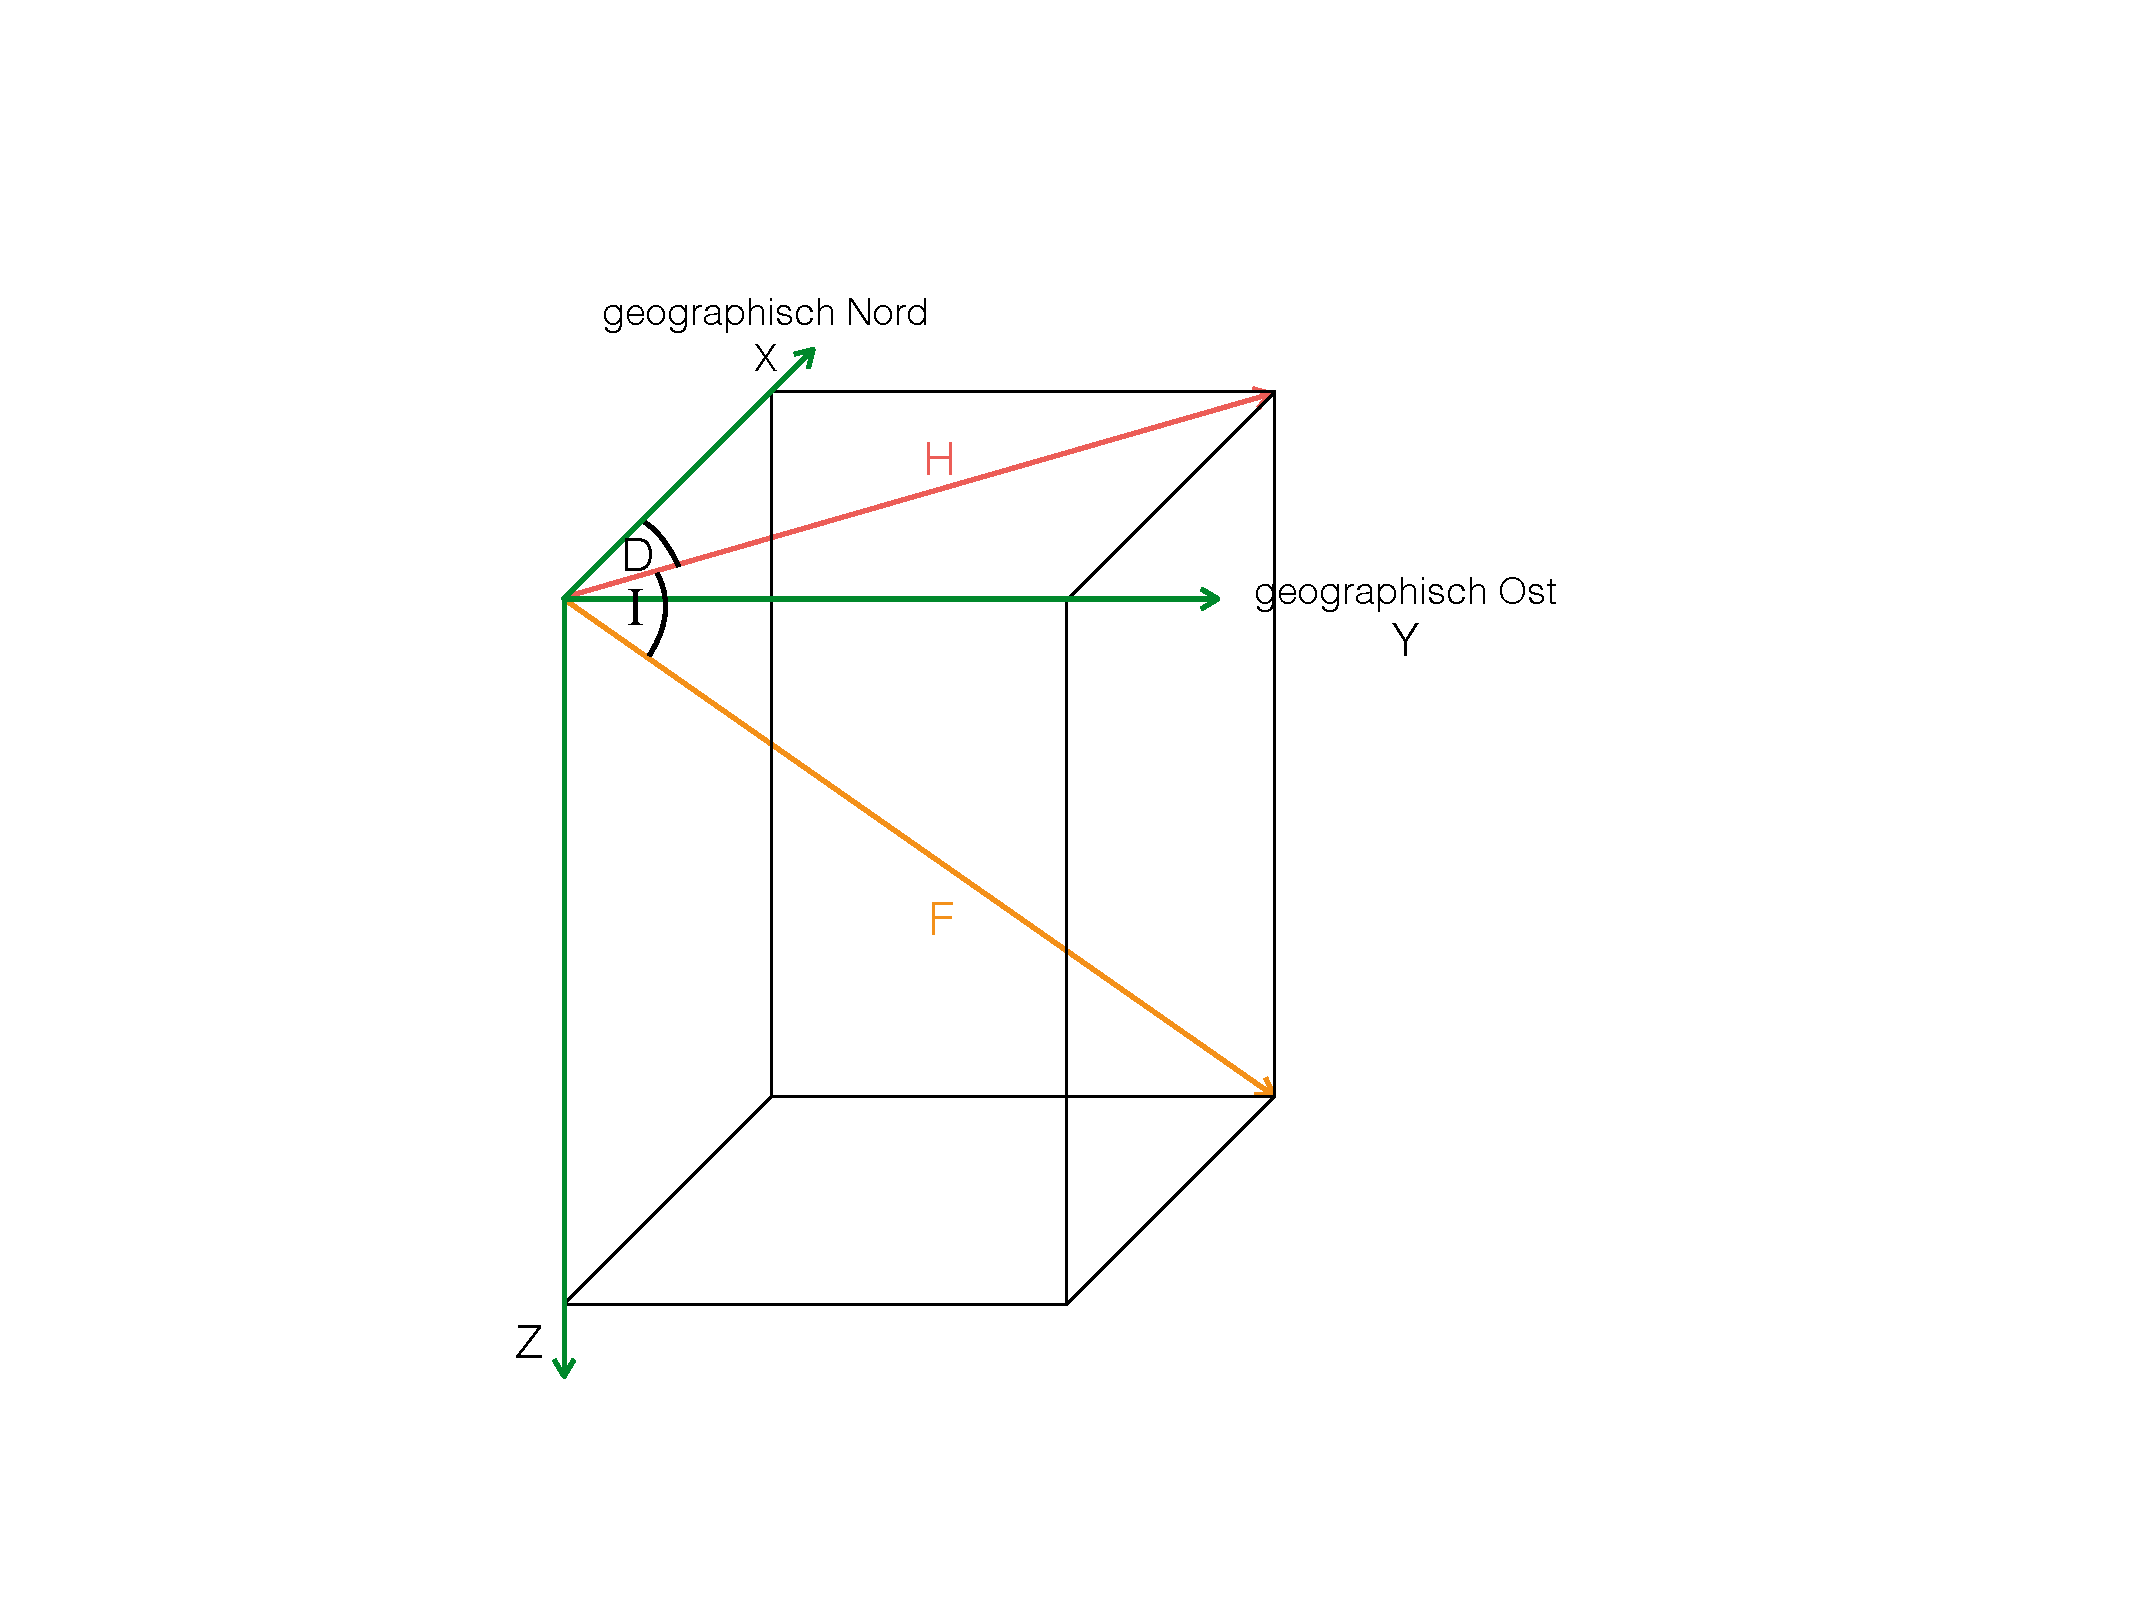
\includegraphics[scale = 0.4]{MagnetikBilder/geomagnetischeFeldelemente}
\end{figure}


Das Erdmagnetfeld lässt sich durch zwei Koordinatensysteme darstellen. $x,y, z$ sind die "`offensichtlichen"' kartesischen Koordinaten, welche geographisch Nord, geographisch Ost und die Tiefe angeben. Hierzu fügen wir nun noch die Kugelkoordinaten, bestehend aus den Winkeln der Deklination und Inklination, sowie des Betrags des Erdmagnetfeldvektors $F$ (\textbf{Totalintensität}). Diese drei Größen lassen sich direkt aus $x,y, z$ berechnen. \begin{equation*}
	tan (D) = \frac{y}{x} \quad \quad tan (I) = \frac{z}{\sqrt{x^2 + y^2}} \quad \quad F = \sqrt{x^2 + y^2 + z^2}
\end{equation*}

Im Feld bei einer Messung werden normalerweise die Vertikalkomponente und die Totalintensität, selten auch die Horizontalkomponente gemessen.


\subsection{Auswertung}
Um auf die Auswertung eingehen zu können, müssen zunächst ein paar Begriffe erklärt werden. 

\subsubsection{Magnetisierung}
Jedes Atom eines Minerals besitzt ein magnetisches Moment mit Betrag und Richtung (Vektor). Das heißt, dass es sich in einem Magnetfeld ausrichtet wie eine Kompassnadel. Die Magnetisierung ist nun die vektorielle Summe aller magnetischen Momente.

\subsubsection{Curie-Temperatur}
Oberhalb der Curie-Temperatur richten sich die magnetischen Momente entlang eines Magnetfeldes aus. Kühlt ein Gestein auf eine Temperatur unterhalb der Curie-Temperatur ab, wird die aktuelle Magnetisierung "`eingefroren"'. Im Folgenden seien noch ein paar Werte der Curie-Temperatur genannt:

\begin{tabular}{ll}
  \textbf{Element} & \textbf{Curie-Temperatur $\vartheta_\text{C}$}\\
  Cobalt & 1121\,$^{\circ}$C\\
  Eisen & 768\,$^{\circ}$C\\
  Nickel & 	360\,$^{\circ}$C\\
  Gadolinium & 19,3\,$^{\circ}$C
\end{tabular} 

\subsubsection{Suszeptibilität}
Die Suszeptibilität gibt an, wie stark sich ein Material "`magnetisieren"' lässt. Sie ist abhängig vom Anteil an Magnetit im Gestein.

\subsubsection{Induzierte Magnetisierung}
Ein Magnetfeld verursacht die Einregelung, also die Ausrichtung der magnetischen Momente. Man spricht dann von induzierter Magnetisierung. Wie stark sich die magnetischen Momente eines Gesteins ausrichten, ist abhängig von der Suszeptibilität.

\subsubsection{Remanente Magnetisierung}
Ist ein Gestein auf eine Temperatur unterhalb der Curie-Temperatur abgekühlt, richten sich die magnetischen Momente nicht mehr am aktuellen Magnetfeld aus. Ihre Magnetisierung ist also bis zum nächsten Erhitzen auf die Curie-Temperatur konstant.

\subsubsection{Königsberger Verhältnis}
Das Königsberger Verhältnis gibt das Verhältnis von induzierter und remanenter Magnetisierung an. \begin{equation*}
	Q = \frac{\text{M}_{\text{rem}}}{\text{M}_{\text{i}}} = \frac{\text{remanente Magnetisierung}}{\text{induzierte Magnetisierung}}
\end{equation*}

Die Größe dieser Zahl $Q$ gibt folglich Aufschluss über die Anteile an remanenter und induzierter Magnetisierung. 

\begin{tabular}{ll}
	$Q \gg 1$ & remanenter Anteil größer als induzierter Anteil  \\
	$Q \ll 1$ & induzierter Anteil größer als remanenter Anteil
\end{tabular}

Diese Zahl spielt vor allem in der Forschung der historischen Geologie eine große Rolle. Der Paläomagnetismus, also die Erhaltung verschiedener Charakteristika des Erdmagnetfeldes im Gestein über die Zeit, gibt Aufschluss über das Alter verschiedener Gesteine und den zeitlichen Verlauf des Erdmagnetfeldes. 
	Aufgrund der sich variierenden Position in Folge des
	Kontinentaldrifts und der mehrfachen Umpolung des
	Erdmagnetfeldes können die in den Gesteinen
	"`gespeicherten"' magnetischen Orientierungen Aufschluss
	über Zeit und Ort der Gesteinsbildung oder der
	Gesteinsablagerung geben.
	
Besonders schön lässt sich das an den Mittelozeanischen Rücken beobachten. Hier tritt aufgrund zweier tektonischer Platten, die sich voneinander weg bewegen, kontinuierlich neues Material aus der Tiefe aus und kühlt langsam ab. Bei einer geomagnetischen Messung sind in Folge deutliche Muster verschiedener Magnetisierungen zu erkennen. 

\begin{figure}[H]
	\includegraphics[width = \textwidth]{MagnetikBilder/PaläomagnetismusMOZ}
    \caption*{Paläomagnetismus an einem Mittelozeanischen Rücken.  \textit{Quelle: Wikipedia}}
\end{figure}











